\documentclass[aspectratio=169]{beamer}
\usepackage[utf8]{inputenc}
\usepackage[T5]{fontenc}
\usepackage{vietnam}
\usepackage{amsmath}
\usepackage{amssymb}
\usepackage{graphicx}
\usepackage{booktabs}
\usepackage{algorithm}
\usepackage{algpseudocode}
\usepackage{multicol}

\usetheme{Madrid}
\usecolortheme{default}

% Tùy chỉnh màu sắc cho các box
\setbeamercolor{block title}{bg=blue!70,fg=white}
\setbeamercolor{block body}{bg=blue!10,fg=black}
\setbeamercolor{block title alerted}{bg=red!70,fg=white}
\setbeamercolor{block body alerted}{bg=red!10,fg=black}
\setbeamercolor{block title example}{bg=teal!60,fg=white}
\setbeamercolor{block body example}{bg=teal!8,fg=black}

\title{Các Kỹ thuật Phân hoạch Lồi cho Hoạch định Chuyển động Robot}
\author{Nhóm 2 Khoa}
\date{\today}

\begin{document}

\frame{\titlepage}

\begin{frame}{Mục tiêu Buổi trình bày}
    \textbf{Các câu hỏi cần làm rõ:}
    \begin{itemize}
        \item Phân hoạch lồi là gì? Tại sao nó quan trọng trong hoạch định chuyển động?
        \item Độ đo xấp xỉ của một vùng lồi được đo lường ra sao?
        \item Trong bài báo, Thuật toán IRIS được sử dụng cụ thể ở đâu, trong trường hợp nào? Có những thuật
              toán nào khác được dùng cho từng trường hợp không?
        \item Các phương pháp được áp dụng trong môi trường 2D như thế nào?
    \end{itemize}
    
    \vspace{1em}
    \begin{alertblock}{Mục tiêu chính}
        Buổi trình bày hôm nay sẽ tập trung giải đáp các câu hỏi trên, cung cấp cái nhìn tổng quan về các kỹ thuật phân hoạch lồi và ứng dụng của chúng.
    \end{alertblock}
\end{frame}

\begin{frame}{Nội dung}
    \tableofcontents
\end{frame}

\section{Các Nguyên tắc Nền tảng}

\begin{frame}{Định nghĩa Phân hoạch Lồi}

    \begin{block}{Định nghĩa}
        \textbf{Phân hoạch lồi (Convex Decomposition)} là quá trình chia một hình học phức tạp (không lồi) thành một tập hợp các \textbf{vùng con lồi} sao cho hợp của chúng khôi phục lại hình ban đầu và các vùng con không chồng lấn nhau (ngoại trừ biên chung).
    \end{block}

    \begin{block}{Công thức}
        Với một miền hình học $P\subset\mathbb{R}^n$, một \textit{phân hoạch lồi} của $P$ là tập hợp $\{P_1, P_2, \dots, P_k\}$ sao cho:
        \[
            P = \bigcup_{i=1}^{k} P_i, \quad
            P_i \cap P_j = \partial P_i \cap \partial P_j \ \text{với mọi } i \ne j,
        \]
        và mỗi $P_i$ là một tập lồi.
        $\partial P_i$ là biên của vùng $P_i$.
    \end{block}

\end{frame}

\begin{frame}{Mục tiêu}

    \textbf{Mục tiêu của Phân hoạch Lồi:}
    \begin{itemize}
        \item Tối thiểu hóa số lượng vùng lồi
        \item Giảm thiểu chồng chéo
        \item Tránh vùng quá ``mảnh'' hoặc ``dài''
    \end{itemize}

\end{frame}

\begin{frame}{Ví dụ về Phân hoạch Lồi Trong 2D}

    \begin{figure}
        \centering
        \begin{tabular}{cc}
            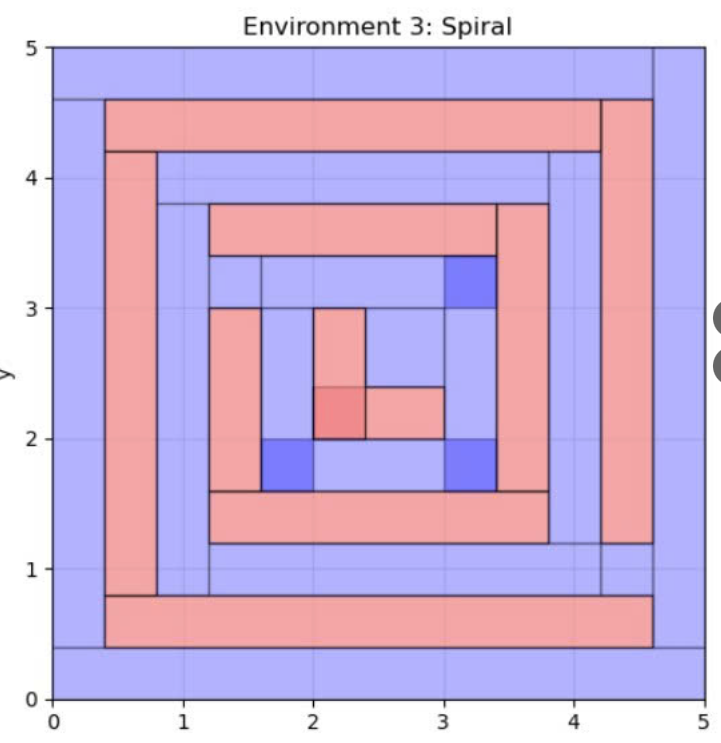
\includegraphics[width=0.2\textwidth]{../imgs/decompose-env3-1.png} &
            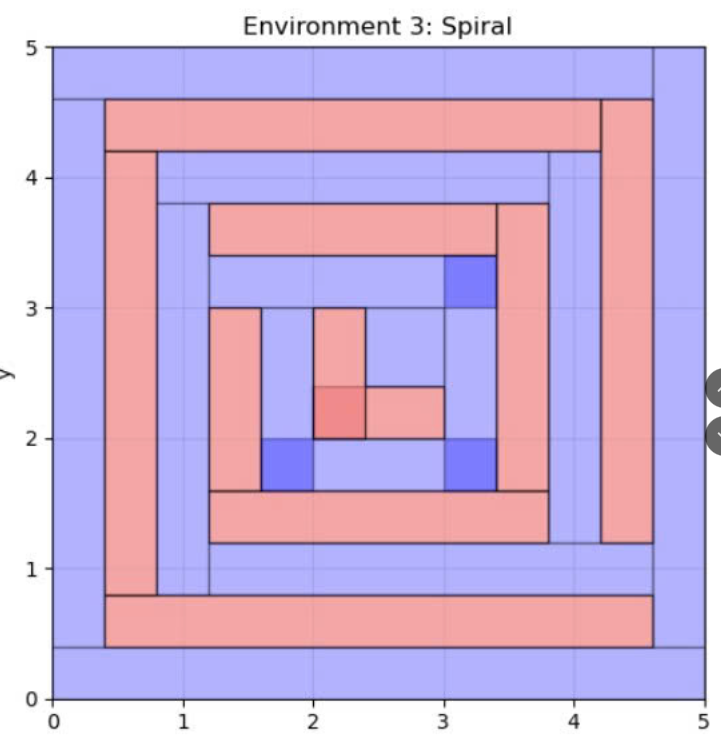
\includegraphics[width=0.2\textwidth]{../imgs/decompose-env3-2.png} \\
            \small (a) Case 1 & \small (b) Case 2 \\[1em]
            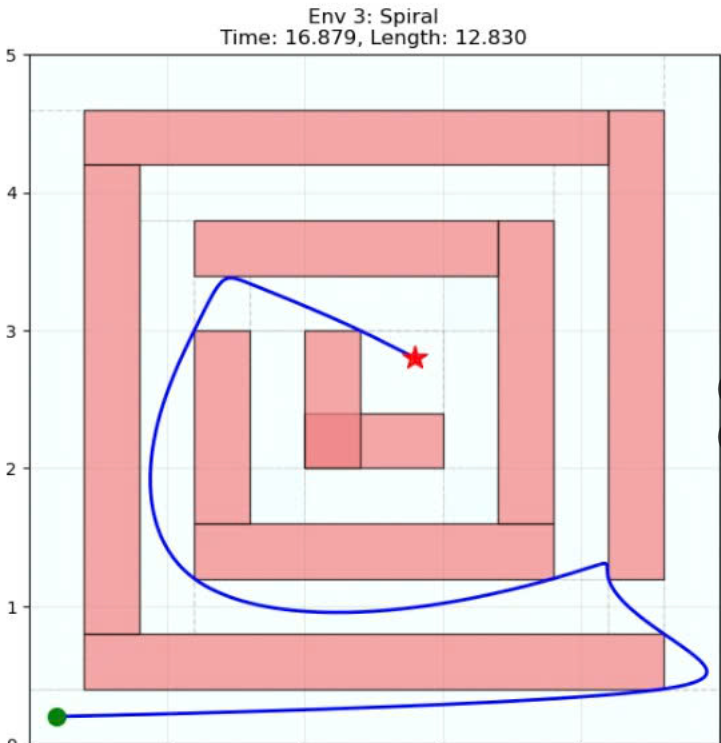
\includegraphics[width=0.2\textwidth]{../imgs/bezier-env3-1.png} &
            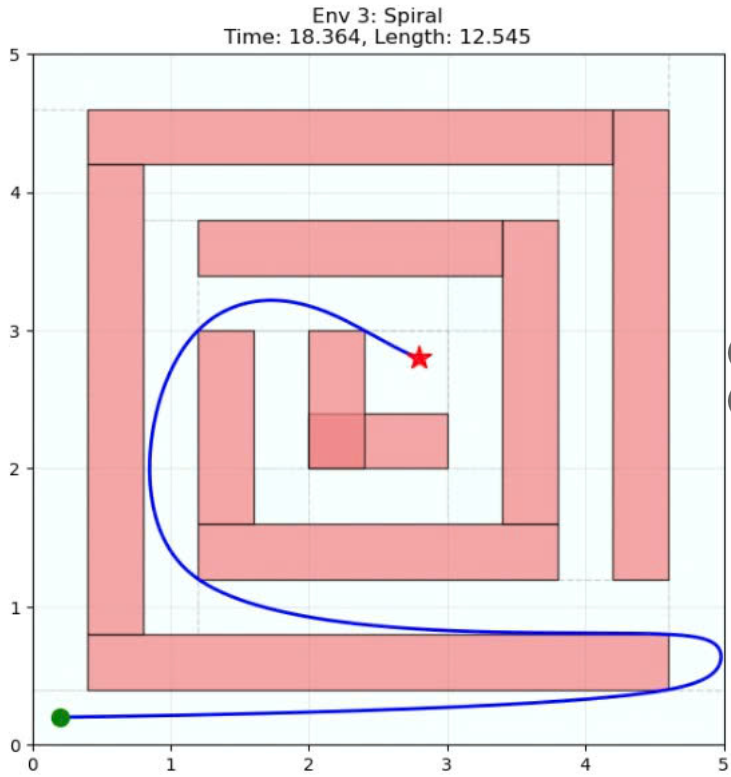
\includegraphics[width=0.2\textwidth]{../imgs/bezier-env3-2.png} \\
            \small (c) Vỏ lồi và khía & \small (d) Kết quả cuối cùng
        \end{tabular}
        \caption{\small Các bước phân hoạch lồi cho đa giác 2D}
    \end{figure}
        
\end{frame}

\begin{frame}{Phân loại Phương pháp}
    \begin{columns}[T]
        \column{0.48\textwidth}
        \textbf{Exact Convex Decomposition (ECD)}
        \begin{itemize}
            \item Thành phần hoàn toàn lồi
            \item Tái tạo chính xác
            \item NP-hard
            \item Số lượng vùng lớn
            \item Chủ yếu có trong lý thuyết
        \end{itemize}

        \column{0.48\textwidth}
        \textbf{Approximate Convex Decomposition (ACD)}
        \begin{itemize}
            \item Gần lồi với dung sai $\tau$
            \item Hiệu quả tính toán cao
            \item Giảm số lượng vùng
            \item Kiểm soát mức chi tiết
            \item Ứng dụng thực tế
        \end{itemize}
    \end{columns}
\end{frame}


\begin{frame}{Các Khái niệm Cơ bản}

    \begin{block}{Định nghĩa các thành phần}
        \begin{itemize}
            \item \textbf{Vỏ Lồi ($H_P$):} Tập lồi nhỏ nhất chứa $P$
                  \[
                      P \text{ lồi} \Leftrightarrow P = H_P
                  \]

            \item \textbf{Khía (Notches):} Đỉnh không trên $H_P$, góc trong $> 180^\circ$

            \item \textbf{Cầu (Bridges):} Cạnh của $\partial H_P$ nối hai đỉnh không liền kề
                  \[
                      \text{BRIDGES}(P) = \partial H_P \setminus \partial P
                  \]

            \item \textbf{Túi (Pockets):} Chuỗi cạnh không thuộc $\partial H_P$
                  \[
                      \text{POCKETS}(P) = \partial P \setminus \partial H_P
                  \]
        \end{itemize}
    \end{block}

\end{frame}

\begin{frame}{Minh họa Các Khái niệm}
    \begin{figure}
        \centering
        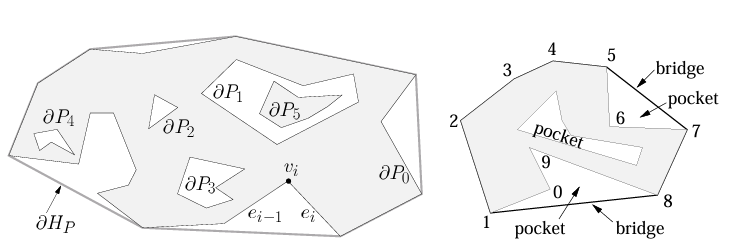
\includegraphics[width=0.8\textwidth]{../imgs/ACD-5.png}
        \caption{\small Vỏ lồi, khía, cầu và túi trong đa giác không lồi}
    \end{figure}
\end{frame}

\section{Phân hoạch Lồi Xấp xỉ (ACD)}

\begin{frame}{Thuật toán ACD - Ý tưởng}

    \textbf{Chiến lược chia để trị đệ quy:}
    \begin{enumerate}
        \item \textbf{Đo độ lõm:} Xác định đỉnh lõm có độ lõm lớn nhất
        \item \textbf{Kiểm tra dung sai:} Nếu độ lõm $< \tau$, kết thúc
        \item \textbf{Giải quyết đỉnh lõm:} Thêm đường cắt, chia đa giác
        \item \textbf{Đệ quy:} Áp dụng cho các thành phần mới
    \end{enumerate}

    \vspace{1em}
    \textbf{Độ phức tạp:} $O(n r^2)$, với $n$ là số đỉnh, $r$ là số đỉnh lõm

\end{frame}

\begin{frame}{Minh họa thuật toán}
    \begin{figure}
        \centering
        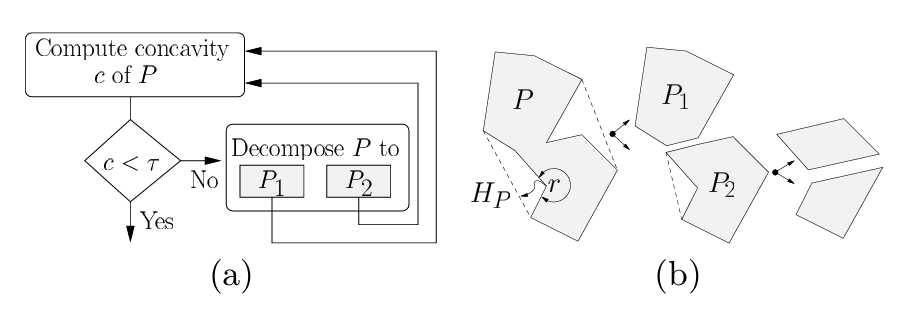
\includegraphics[width=0.8\linewidth]{../imgs/ACD-1.png}
        \caption{Quá trình đệ quy tiếp tục cho đến khi đạt đến giới hạn độ lõm đầu vào của người dùng $\tau$.}
    \end{figure}
\end{frame}

\begin{frame}{Ví dụ về Giải quyết Độ lõm}
    \vspace{0.5em}
    \textbf{Các trường hợp xử lý:}
    
    \textbf{(a)} Gộp biên vào đa giác

    \textbf{(b)} Tách đa giác thành hai

    \textbf{(c)} Độ lõm thay đổi sau phân rã

    \vspace{0.2cm}
    Quá trình tiếp tục đến khi độ lõm $\leq \tau$

     \centering
    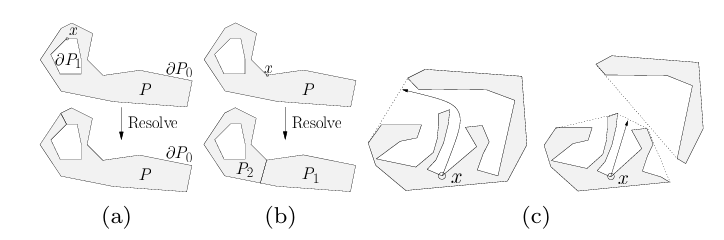
\includegraphics[width=0.7\textwidth]{../imgs/ACD-3.png}
\end{frame}




\begin{frame}{Các Thước đo Độ lõm}
    \centering
    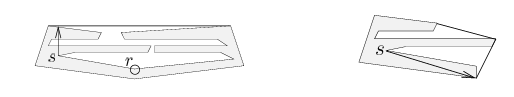
\includegraphics[width=0.8\linewidth]{../imgs/ACD-2.png}

    \vspace{0.5em}
    \textbf{SL-Concavity:} Khoảng cách Euclid đến cầu nối (bridge).
    \begin{itemize}
        \item[\textcolor{teal}{+}] Nhanh
        \item[\textcolor{red}{--}] Không đảm bảo tính đơn điệu
    \end{itemize}

\end{frame}

\begin{frame}{Các Thước đo Độ lõm}
    \centering
    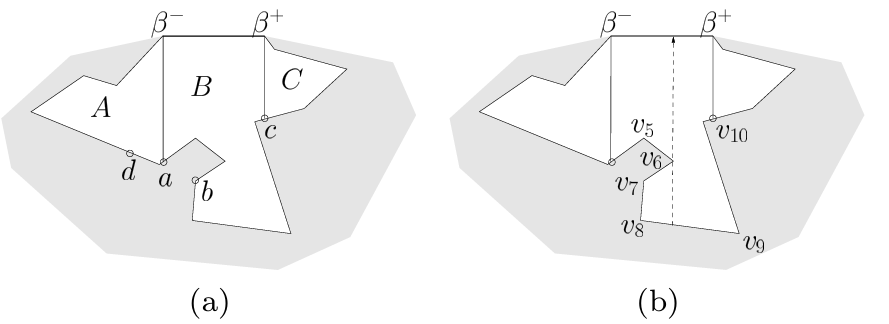
\includegraphics[width=0.7\textwidth]{../imgs/sp_concavity.png}

    \vspace{0.5em}
    \textbf{SP-Concavity:} Đường đi ngắn nhất trong túi (pocket) đến cầu nối tương ứng.
    \begin{itemize}
        \item[\textcolor{red}{--}] Chậm hơn
        \item[\textcolor{teal}{+}] Đảm bảo tính đơn điệu
        \item[\textcolor{teal}{+}] Xử lý tất cả đặc điểm lõm quan trọng
    \end{itemize}

\end{frame}

\begin{frame}{Các Thước đo Độ lõm}
    \centering
    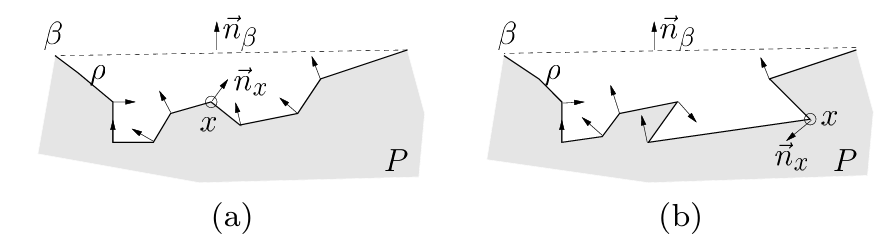
\includegraphics[width=0.7\linewidth]{../imgs/ACD-6.png}
    
    \vspace{0.5em}
    \textbf{H-Concavity:} Lai ghép SL và SP - Mặc định dùng SL, chuyển sang SP khi phát hiện không đơn điệu (kiểm tra: $n_\beta \cdot n_i < 0$).

\end{frame}

\section{IRIS Algorithm}

\begin{frame}{IRIS - Ý tưởng Chính}

    \textbf{IRIS:} Iterative Regional Inflation by Semidefinite Programming
    
    \textbf{Câu hỏi cốt lõi:} Với điểm mầm (seed), vùng lồi lớn nhất là gì?

    \vspace{1em}
    \textbf{Quy trình lặp 4 bước:}
    \begin{enumerate}
        \item Khởi tạo hình cầu \underline{rất nhỏ} tại seed
        \item Tìm siêu phẳng phân cách (QP)
        \item Tìm ellipsoid nội tiếp cực đại (SDP)
        \item Lặp lại đến hội tụ
    \end{enumerate}

    \vspace{0.5em}
    \textbf{Output:} Một vùng lồi lớn nhất từ seed point

\end{frame}
\begin{frame}{IRIS Bước 2: Tìm Siêu phẳng Phân cách}
    
    \textbf{Mục tiêu:} Tìm siêu phẳng phân tách ellipsoid với obstacles
    
    \begin{columns}[c]
        \column{0.5\textwidth}
        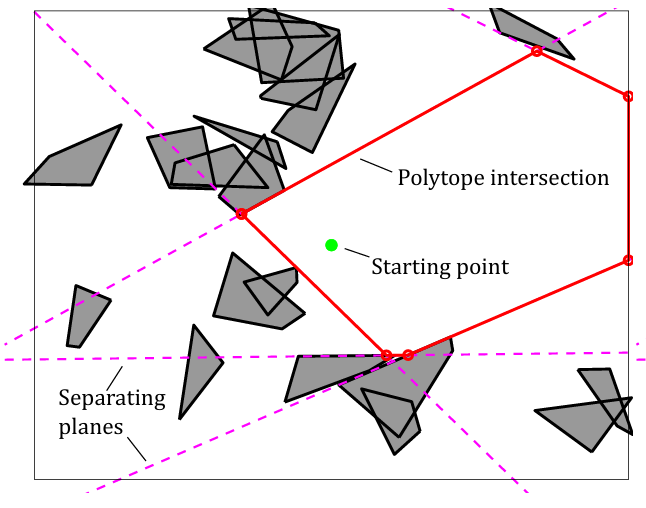
\includegraphics[width=\textwidth]{../imgs/iris_algo_1.png}
        
        \column{0.5\textwidth}
        \vspace{0.5em}
        \textbf{Giải pháp - Thuật toán tham lam:}
        \begin{enumerate}
            \item Bắt đầu từ obstacle gần ellipsoid nhất
            \item Tìm điểm trên obstacle gần nhất
            \item Tính siêu phẳng $a_j^\top x \geq b_j$
            \item Kiểm tra tất cả obstacles khác $o_k$:
            
            Nếu $a_j^\top v \geq b_j$ $\forall v \in o_k$
            
            $\Rightarrow$ Loại $o_k$ (đã bị phân tách)
            \item Lặp lại cho obstacles còn lại
        \end{enumerate}

        \vspace{0.3em}
        {\small
        \textbf{Ký hiệu:}
        $o_j$: obstacle j \\
        $v$: đỉnh của obstacle\\
        $a_j, b_j$: tham số siêu phẳng
        }
    \end{columns}

\end{frame}

\begin{frame}{IRIS - Tìm obstacle Gần nhất}

        \textbf{Biến đổi không gian:}
        
        \vspace{0.5em}
        $\Rightarrow$ Biến đổi về không gian quả cầu đơn vị:
        
        \begin{itemize}
            \item Ellipsoid: $\mathcal{E} = \{C\tilde{x} + d : \|\tilde{x}\|_2 \leq 1\}$
            \item Quả cầu: $\tilde{\mathcal{E}} = \{\tilde{x} : \|\tilde{x}\| \leq 1\}$
            \item Obstacle: $\tilde{o}_j = \text{ConvexHull}(\tilde{v}_{j,1}, \ldots, \tilde{v}_{j,m})$
            \item Với $\tilde{v}_{j,k} = C^{-1}(v_{j,k} - d)$
        \end{itemize}

        Khi này khoảng cách đến ellipsoid tương đương với khoảng cách đến gốc tọa độ trong không gian biến đổi.
        
        \vspace{0.3em}
        {\small
        \textbf{Ký hiệu:}
        $C$: ma trận xác định hình dạng ellipsoid,
        $d$: tâm ellipsoid,
        $v_{j,k}$: đỉnh thứ $k$ của obstacle $j$ trong không gian gốc,
        $\tilde{v}_{j,k}$: đỉnh sau biến đổi
        }
\end{frame}

\begin{frame}{IRIS - Bài toán QP cho Điểm Gần nhất}
    
    \begin{block}{QP Problem}
        \small
        Tìm điểm gần nhất đến gốc tọa độ trong không gian biến đổi:
        \[
            \begin{aligned}
                \min_{\tilde{x}, w} \quad & \|\tilde{x}\|^2                \\
                \text{s.t.} \quad         & [\tilde{v}_{j,1}, \tilde{v}_{j,2}, \ldots, \tilde{v}_{j,m}]w = \tilde{x} \\
                                          & \sum_{i=1}^{m} w_i = 1 \\
                                          & w_i \geq 0
            \end{aligned}
        \]
        
        $\tilde{x}$ là tổ hợp lồi của các đỉnh $\tilde{v}_{j,k}$ gần gốc nhất
    \end{block}

    \vspace{0.5em}
    \textbf{Biến đổi ngược:} $x^* = C\tilde{x}^* + d$ là điểm gần ellipsoid nhất trên obstacle $o_j$

    \vspace{0.3em}
    {\small
    \textbf{Ký hiệu:}
    $\tilde{x}$: điểm cần tìm trong không gian biến đổi,
    $w = [w_1, \ldots, w_m]$: hệ số tổ hợp lồi,
    $\tilde{v}_{j,k}$: đỉnh thứ $k$ của obstacle $j$ sau biến đổi,
    $m$: số đỉnh của obstacle
    }

    
    
\end{frame}

\begin{frame}{IRIS - Tính Siêu phẳng Tiếp tuyến}
    \begin{columns}[c]
        \column{0.5\textwidth}
        
        \textbf{Biểu diễn ngược của Ellipsoid:}
        \[
            \mathcal{E} = \{x : (x-d)^\top C^{-1}C^{-\top}(x-d) \leq 1\}
        \]

        \vspace{0.5em}
        \begin{block}{Tính pháp tuyến}
            \small
            Gradient của hàm rào cản tại $x^*$:
            \[
                a_j = \nabla_x[(x-d)^\top C^{-1}C^{-\top}(x-d)]|_{x^*}
            \]
            \[
                = 2C^{-1}C^{-\top}(x^* - d)
            \]
            
            Hệ số tự do:
            \[
                b_j = a_j^\top x^*
            \]
        \end{block}

        \column{0.45\textwidth}
        % 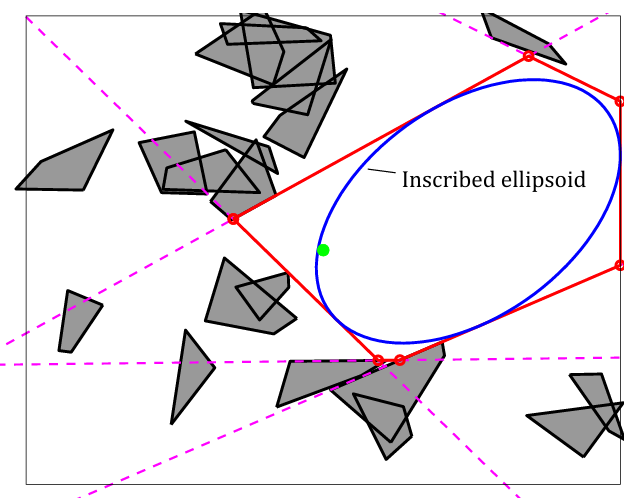
\includegraphics[width=\textwidth]{../imgs/iris_2.png}
        
        \vspace{0.5em}
        \textbf{Kết quả:}
        
        Siêu phẳng $a_j^\top x = b_j$ tiếp xúc với $\mathcal{E}_{\alpha^*}$ tại $x^*$ và phân tách $\mathcal{E}$ khỏi $o_j$
        
        \vspace{0.3em}
        Chọn chiều: $a_j^\top x \geq b_j$ $\forall x \in o_j$
    \end{columns}
\end{frame}

    
\begin{frame}{IRIS Bước 3: Ellipsoid Nội tiếp Cực đại}
    \begin{columns}[c]
        \column{0.45\textwidth}
        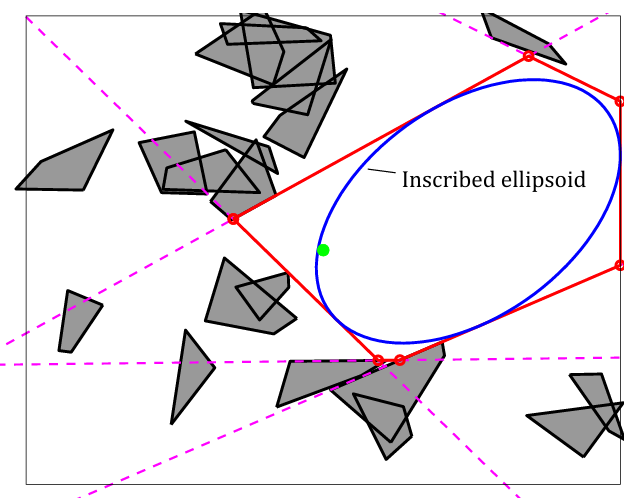
\includegraphics[width=\textwidth]{../imgs/iris_2.png}

        \column{0.5\textwidth}
        
        \textbf{Đầu vào:} Tập siêu phẳng $\{a_i^\top x \geq b_i\}_{i=1}^m$

        \begin{block}{SDP Problem}
            \small
            \[
                \begin{aligned}
                    \max_{C,d} \quad  & \log \det C                            \\
                    \text{s.t.} \quad & \|a_i^\top C\|_2 + a_i^\top d \leq b_i \\
                                      & C \succeq 0
                \end{aligned}
            \]

            Tối đa hóa thể tích ellipsoid nội tiếp đa diện
        \end{block}

        \vspace{0.5em}
        \textbf{Ràng buộc:}
        
        $\|a_i^\top C\|_2 + a_i^\top d \leq b_i$ đảm bảo ellipsoid nằm trong nửa không gian $a_i^\top x \leq b_i$
    \end{columns}
\end{frame}


\begin{frame}{IRIS - Phân tích Độ phức tạp}

    \textbf{Độ phức tạp mỗi vòng lặp:}
    
    \vspace{0.5em}
    \begin{block}{SeparatingHyperplanes: $O(m \cdot n \cdot k)$}
        \small
        \begin{itemize}
            \item $m$: số lượng obstacles
            \item $n$: số đỉnh trung bình mỗi obstacle
            \item $k$: số vòng lặp QP để tìm điểm gần nhất (CVXPY solve)
        \end{itemize}
    \end{block}

    \vspace{0.3em}
    \begin{block}{InscribedEllipsoid: $O(h^3)$}
        \small
        \begin{itemize}
            \item SDP với $h$ ràng buộc siêu phẳng
            \item Interior point method: $O(h^3)$ mỗi vòng lặp SDP
        \end{itemize}
    \end{block}

\end{frame}

\begin{frame}{IRIS - Độ phức tạp Tổng thể}

    \begin{block}{Công thức tổng quát}
        \[
            O(T \cdot (m \cdot n \cdot k + h^3))
        \]
        
        \small
        Với $T$: số vòng lặp IRIS (thường 4-8 vòng)
    \end{block}

    \vspace{1em}
    \textbf{Giải thích các thành phần:}
    \begin{itemize}
        \item \textbf{$T$:} Số vòng lặp IRIS - thường hội tụ nhanh (4 - 8)
        \item \textbf{$m \cdot n \cdot k$:} Chi phí tìm siêu phẳng phân cách
        \item \textbf{$h^3$:} Chi phí giải SDP cho ellipsoid nội tiếp cực đại
    \end{itemize}

    \vspace{0.5em}
    \textbf{Nhận xét:}
    \begin{itemize}
        \item Độ phức tạp tăng tuyến tính theo số obstacles ($m$)
        \item Phần SDP ($h^3$) thường là cố định do số lượng siêu phẳng không thay đổi nhiều
        \item Hội tụ nhanh ($T$ nhỏ) làm thuật toán khả thi trong thực tế
    \end{itemize}

\end{frame}

\begin{frame}{IRIS - Độ phức tạp Thực nghiệm}
    \begin{figure}
        \centering
        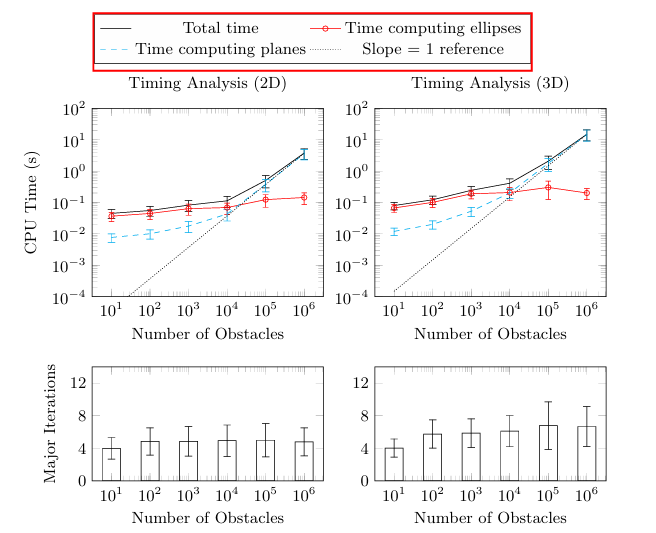
\includegraphics[width=0.5\textwidth]{../imgs/time-iris.png}
        \caption{\small Thời gian thực thi IRIS tăng tuyến tính với số lượng obstacles.}
    \end{figure}
\end{frame}


\begin{frame}{IRIS - Đặc tính}

    \textbf{Thuộc tính chính:}
    \begin{itemize}
        \item \textbf{Loại:} Phương pháp xấp xỉ
        \item \textbf{Hội tụ:} 4-8 vòng lặp
        % \item \textbf{Độ phức tạp:} Tuyến tính theo số obstacles
    \end{itemize}

    \vspace{1em}
    \textbf{Xử lý obstacles không lồi:}
    \begin{itemize}
        \item \textbf{Work space:} Bao lồi hoặc phân hoạch trước
        \item \textbf{Configuration space:} IRIS-NP, C-IRIS
    \end{itemize}

\end{frame}

\section{Visibility Clique Cover (VCC)}

\begin{frame}{VCC - Giải quyết Vấn đề Seeding}

    \textbf{Hạn chế của IRIS:}
    \begin{itemize}
        \item IRIS gia đình các obstacles là lồi, nên cần 1 bước tiền xử lý trước
        \item Cần chọn seed points tốt (người dùng tự chọn)
        % \item Việc lấy mầm ngẫu nhiên không hiệu quả
    \end{itemize}

    \vspace{1em}
    \textbf{Giải pháp VCC:}
    \begin{itemize}
        \item Tự động hóa quy trình seeding
        \item Sử dụng cấu trúc toàn cục của không gian tự do
    \end{itemize}

\end{frame}

\begin{frame}{VCC - Giải quyết Vấn đề Seeding}
    \textbf{Quy trình 4 bước:}
    \begin{enumerate}
        \item Lấy mẫu $n$ điểm trong $C_{free}$
        \item Xây dựng đồ thị khả kiến (visibility graph)
        \item Tìm lớp phủ clique (MAXCLIQUE + ILP)
        \item Khởi tạo ellipsoid và lấp đầy (IRIS-like)
    \end{enumerate}

    \vspace{0.5em}
    \textbf{Ý tưởng cốt lõi:} Điểm ``nhìn thấy'' nhau $\Rightarrow$ có khả năng cùng vùng lồi

    \vspace{0.5em}
    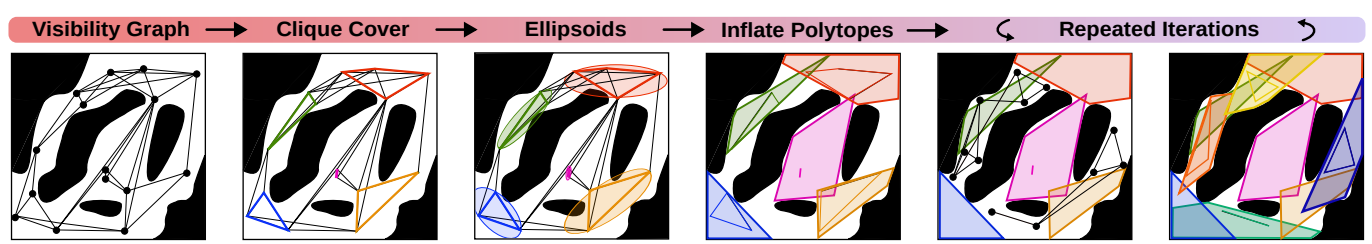
\includegraphics[width=\textwidth]{../imgs/VCC.png}

\end{frame}


\begin{frame}{VCC - Bước 1: Lấy mẫu \& Xây dựng Đồ thị Khả kiến}
    \begin{columns}[c]
        \column{0.45\textwidth}
        \centering
        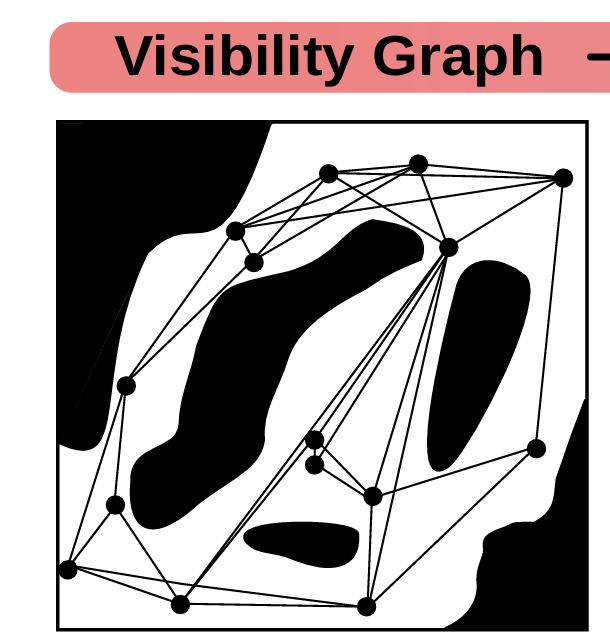
\includegraphics[width=\textwidth]{../imgs/VCC-1.png}

        \column{0.5\textwidth}
        \textbf{Visibility Graph Construction:}
        \begin{itemize}
            \item Lấy mẫu $n$ điểm ngẫu nhiên trong $C_{free}$
            \item Tạo cạnh giữa hai điểm nếu đoạn thẳng nối chúng không va chạm
            \item Xây dựng đồ thị khả kiến (visibility graph)
        \end{itemize}

        \vspace{0.5em}
        \begin{exampleblock}{Định nghĩa}
            \textbf{Visibility graph:} Đồ thị có cạnh nối hai đỉnh khi đoạn thẳng nối chúng nằm hoàn toàn trong không gian tự do
        \end{exampleblock}
    \end{columns}
\end{frame}

\begin{frame}{VCC - Bước 2: Tìm Lớp phủ Clique}
    \begin{columns}[c]
        \column{0.45\textwidth}
        \centering
        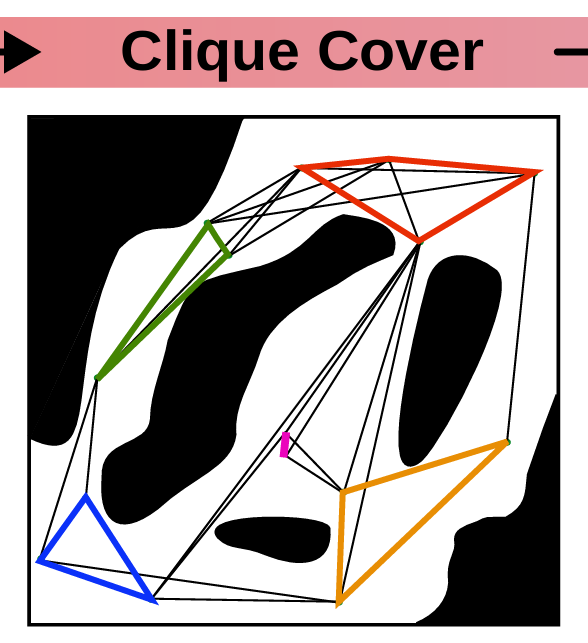
\includegraphics[width=\textwidth]{../imgs/VCC-2.png}

        \column{0.5\textwidth}
        \textbf{Clique Cover Problem:}
        \begin{itemize}
            \item Tìm tập hợp các clique lớn (đồ thị con đầy đủ)
            \item Sử dụng MAXCLIQUE algorithm
            \item Giải bài toán Integer Linear Programming (ILP)
        \end{itemize}

        \vspace{0.5em}
        \textbf{Ý tưởng cốt lõi:}
        
        Các điểm "nhìn thấy" nhau có khả năng nằm trong cùng một vùng lồi
        
        \vspace{0.2cm}
        \textit{Con đường thẳng = an toàn}
    \end{columns}
\end{frame}

\begin{frame}{VCC - Bước 3: Khởi tạo Ellipsoid}
    \begin{columns}[c]
        \column{0.45\textwidth}
        \centering
        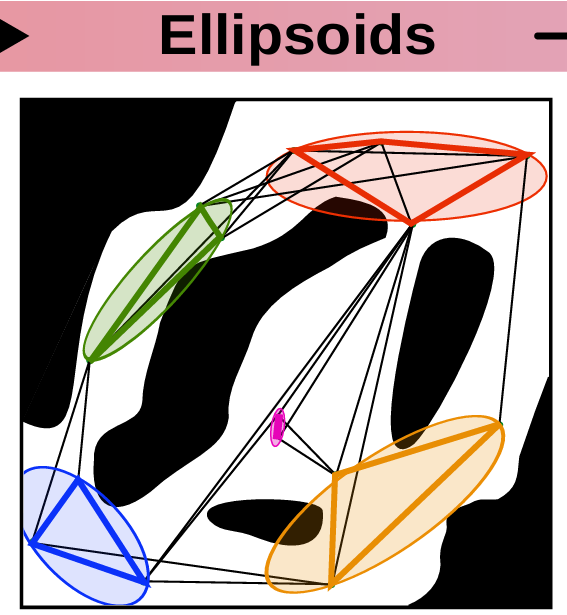
\includegraphics[width=\textwidth]{../imgs/VCC-3.png}

        \column{0.5\textwidth}
        \textbf{Ellipsoid Initialization:}
        \begin{itemize}
            \item Tính ellipsoid có thể tích nhỏ nhất bao quanh tất cả điểm trong clique
            \item Cung cấp tâm (seed point) cho bước tiếp theo
            \item Xác định hình dạng ban đầu (các trục chính)
        \end{itemize}

        \vspace{0.5em}
        \textbf{Lợi ích:}
        
        Ellipsoid đã được "thông báo" về hình học cục bộ
        
        $\Rightarrow$ Hiệu quả hơn IRIS tiêu chuẩn
    \end{columns}
\end{frame}


\begin{frame}{VCC - Bước 4: Lấp đầy thành Đa diện}
    \begin{columns}[c]
        \column{0.45\textwidth}
        \centering
        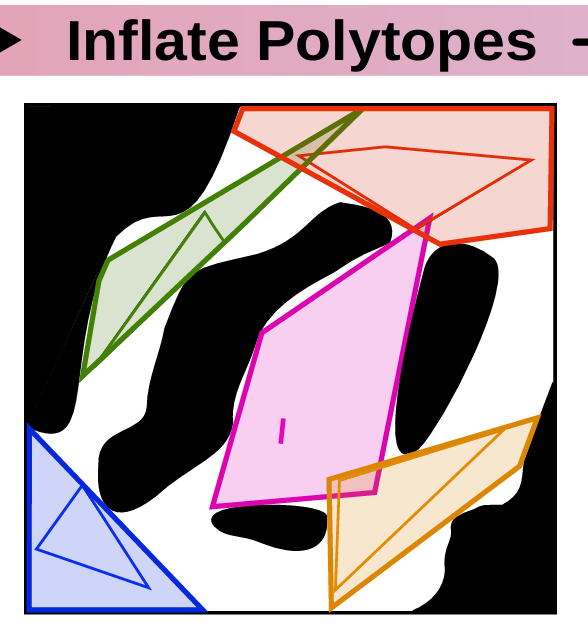
\includegraphics[width=\textwidth]{../imgs/VCC-4.png}

        \column{0.5\textwidth}
        \textbf{Inflation Process:}
        \begin{itemize}
            \item Sử dụng thuật toán tương tự IRIS
            \item Một vòng lặp duy nhất (thay vì nhiều vòng)
            \item Tạo đa diện lồi cuối cùng từ ellipsoid
        \end{itemize}

        \vspace{0.5em}
        \textbf{Hiệu quả cao hơn IRIS:}
        
        Ellipsoid ban đầu đã được ``thông báo'' về hình học cục bộ
        
        $\Rightarrow$ Loại bỏ nhiều vòng lặp tốn kém
    \end{columns}
\end{frame}

\begin{frame}{VCC - Bước 5: Lặp lại và Hội tụ}
    \begin{columns}[c]
        \column{0.45\textwidth}
        \centering
        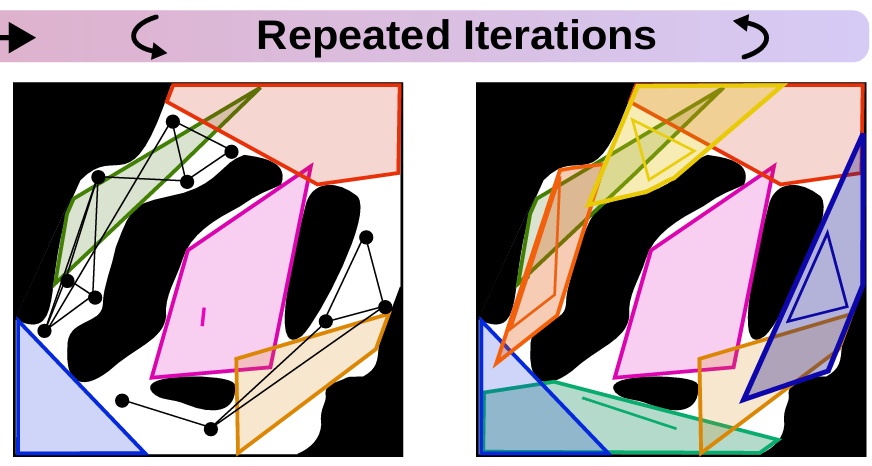
\includegraphics[width=\textwidth]{../imgs/VCC-5.png}

        \column{0.5\textwidth}
        \textbf{Iteration Process:}
        \begin{itemize}
            \item Lấy mẫu mới từ không gian trống còn lại
            \item Lặp lại các bước 1-4 cho vùng chưa phủ
            \item Tiếp tục đến khi đạt độ phủ $\alpha$ đủ
        \end{itemize}

        \vspace{0.5em}
        \textbf{Điều kiện dừng - Quá trình kết thúc khi:}
        \begin{itemize}
            \item Đạt độ phủ mong muốn $\alpha$
            \item Không còn không gian đáng kể để phủ
            \item Số vùng lồi đã đủ cho ứng dụng
        \end{itemize}
    \end{columns}
\end{frame}


\begin{frame}{VCC - Đặc tính và Ưu điểm}

    \textbf{Đặc tính:}
    \begin{itemize}
        \item \textbf{Loại:} Phương pháp xấp xỉ
        \item \textbf{Mục tiêu:} Tối thiểu hóa số vùng với độ phủ $\alpha$
        \item \textbf{Phương pháp:} Lai ghép hình học và ILP
    \end{itemize}

    \vspace{1em}
    \textbf{Ưu điểm:}
    \begin{itemize}
        \item Tự động hóa hoàn toàn
        \item Không phụ thuộc hình dạng obstacles
        \item Sử dụng kiểm tra va chạm chung
    \end{itemize}

\end{frame}

\section{Ứng dụng trong GCS}

\begin{frame}{Vai trò trong Graph of Convex Sets}

    \textbf{Khuôn khổ GCS:}
    
    Yêu cầu phân hoạch lồi trước khi hoạch định chuyển động

    \vspace{1em}
    \textbf{Vai trò phân hoạch:}
    \begin{itemize}
        \item Các vùng lồi = đỉnh trong đồ thị $G$
        \item Chất lượng phân hoạch $\Rightarrow$ hiệu suất GCS
        \item Phân hoạch kém $\Rightarrow$ đồ thị phức tạp
    \end{itemize}

    \vspace{0.5em}
    \begin{alertblock}{Chuỗi phụ thuộc}
        Thuật toán phân hoạch tiên tiến $\Rightarrow$ GCS khả thi $\Rightarrow$ Giải quyết bài toán DOF cao
    \end{alertblock}

\end{frame}

\begin{frame}{Phương pháp theo Môi trường \& Độ phức tạp}

    \begin{columns}[c]

        \column{0.5\textwidth}
        \textbf{2D đơn giản:}
        \begin{itemize}
            \item 2D : Manual Exact Decomposition thanh cac da giac loi.
            \item Maze: Grid $50 \times 50$
        \end{itemize}
    
        \vspace{0.8em}
        \textbf{3D Quadrotor:}
        \begin{itemize}
            \item Box Decomposition
            \item Thu nhỏ theo robot radius
        \end{itemize}
    
        \vspace{0.8em}
        \textbf{High-DOF (7/14-DOF):}
        \begin{itemize}
            \item IRIS Approximate
            \item Seed qua Inverse Kinematics hoặc thu cong.
            \item Dual arms: Tích Descartes
        \end{itemize}

        \column{0.5\textwidth}
        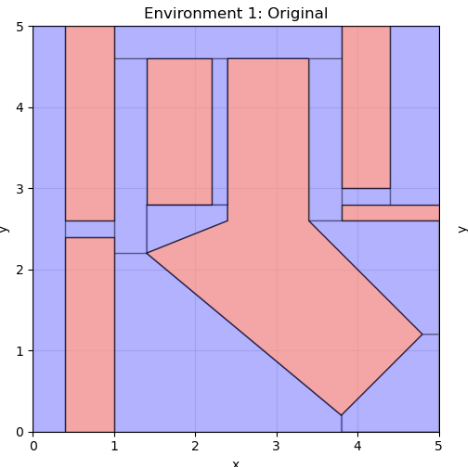
\includegraphics[width=\textwidth]{../imgs/2d-decompose-ex.png}
        
    \end{columns}

\end{frame}

\begin{frame}{Chi tiết hiện thực 2D - Phân hoạch Chính xác}
    \begin{columns}[c]
        \column{0.45\textwidth}
        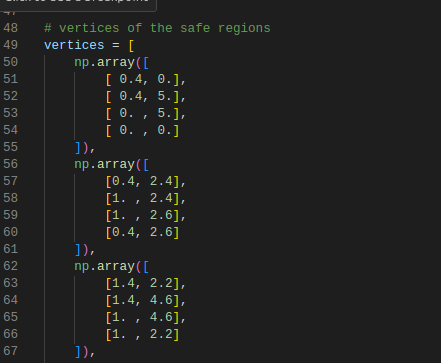
\includegraphics[width=\textwidth]{../imgs/2d-decompose.png}

        \column{0.5\textwidth}
        \textbf{Two-Dimensional Example}
        
        \textbf{12 vùng lồi V-polytope}

        \vspace{0.3cm}
        Chuyển đổi sang dạng H-polytope (hyperplanes):
        \[
            \mathcal{R}_i = \{x \in \mathbb{R}^2 : A_i x \leq b_i\}
        \]

        \vspace{0.3cm}
        Sử dụng \texttt{ConvexHull} algorithm

        \vspace{0.3cm}
        \textbf{Kết quả:} Phù hợp hoàn hảo với GCS framework
    \end{columns}
\end{frame}

\begin{frame}{Ví dụ Maze - Grid Decomposition}
    \begin{columns}[c]
        \column{0.45\textwidth}
        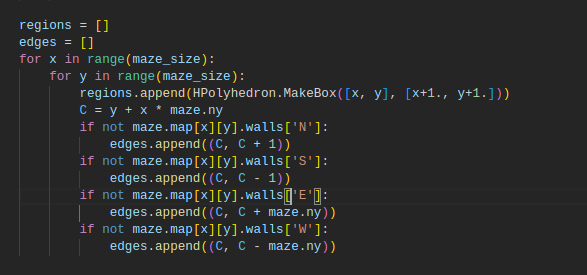
\includegraphics[width=\textwidth]{../imgs/maze-decompose.png}

        \column{0.5\textwidth}
        \textbf{Maze Planning}
        
        \textbf{Lưới đều $50 \times 50$}

        \vspace{0.3cm}
        Mỗi ô = vùng lồi $Q_i$

        \vspace{0.3cm}
        \textbf{Graph connectivity:}
        \begin{itemize}
            \item Dựa trên cấu trúc tường
            \item Hai ô kề không tường $\Rightarrow$ có cạnh
            \item Đơn giản nhưng kém hiệu quả khi kích thước lưới lớn
        \end{itemize}
    \end{columns}
\end{frame}

\begin{frame}{Ví dụ 3D Quadrotor - Chi tiết Box Decomposition}

    \textbf{Thuật toán chia nhỏ không gian:}
    \begin{itemize}
        \item \textbf{Phòng (Indoor):} Hộp duy nhất cho mỗi ô
            %   \[
            %       \text{size} = 2.5 - (\text{wall\_offset} + \text{quad\_radius})
            %   \]

        \item \textbf{Ngoài trời (Outdoor):}
              \begin{itemize}
                  \item \textit{Không cây:} Hộp lớn bao phủ toàn bộ
                  \item \textit{Có cây:} 4 hộp xung quanh (trên, dưới, trái, phải)
              \end{itemize}

        \item \textbf{Khe hở tường:}
              \begin{itemize}
                  \item \textit{Cửa:} Hộp hẹp cao
                  \item \textit{Cửa sổ:} 1-2 hộp nhỏ  
                  \item \textit{Không tường:} Hộp lớn nối phòng
              \end{itemize}
    \end{itemize}

\end{frame}

\begin{frame}{High-DOF: KUKA 7-DOF \& Dual Arms 14-DOF}

    \textbf{Giải pháp IRIS-based:}
    \begin{itemize}
        \item Sử dụng \texttt{IrisInConfigurationSpace} (C-IRIS)
        \item Xử lý chướng ngại vật không lồi trong C-space
        \item Sinh đa diện lồi $Q_i$ quanh seed points
        \item Song song hóa cho nhiều seed khác nhau
    \end{itemize}

    \vspace{1em}
    \textbf{Dual Arms: Kết hợp không gian}
    
    Tích Descartes hoặc hợp lồi của các vùng từ từng cánh tay riêng lẻ

\end{frame}

% \begin{frame}{Hạn chế và Cơ hội Cải tiến}

%     \begin{alertblock}{Vấn đề Seeding thủ công}
%         \begin{itemize}
%             \item IRIS cần seed points được chọn thủ công
%             \item Sử dụng Inverse Kinematics để tạo seed
%             \item Không tự động, phụ thuộc kinh nghiệm người dùng
%         \end{itemize}
%     \end{alertblock}

%     % \begin{exampleblock}{Cơ hội với VCC}
%     %     \begin{itemize}
%     %         \item VCC tự động hóa hoàn toàn việc seeding
%     %         \item Không cần can thiệp thủ công
%     %         \item Phù hợp cho các hệ thống tự động
%     %     \end{itemize}
%     % \end{exampleblock}

%     \begin{block}{Ý nghĩa thực tiễn}
%         \textbf{Sự thành công của IRIS trong C-space nhiều chiều làm cho GCS khả thi cho robot thế giới thực}
%     \end{block}

% \end{frame}

\begin{frame}{Kết luận}

    \textbf{Ứng dụng theo môi trường:}
    \begin{itemize}
        \item 2D: Exact decomposition
        \item 3D: Box/Grid decomposition
        \item High-DOF: IRIS-based approximation
    \end{itemize}

    \vspace{1em}
    \begin{alertblock}{Kết nối với GCS}
        \textbf{GCS framework} phụ thuộc hoàn toàn vào chất lượng phân hoạch
    \end{alertblock}

\end{frame}

\section{Demo}

% \begin{frame}{Demo 1}
%     \begin{figure}
%         \centering
%         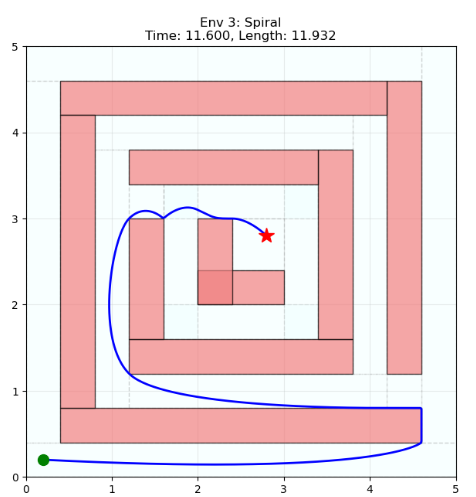
\includegraphics[width=0.45\textwidth]{../imgs/spriral-case2.png}
%         % \caption{}
%     \end{figure}
% \end{frame}

% \begin{frame}{Demo 2}
%     \begin{columns}[c]
%         \column{0.48\textwidth}
%         \begin{figure}
%             \centering
%             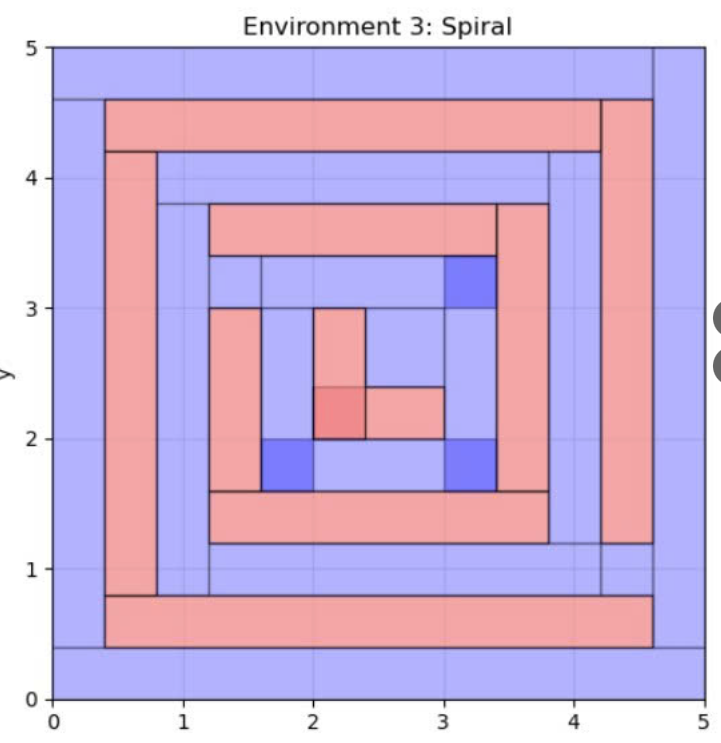
\includegraphics[width=0.8\textwidth]{../imgs/decompose-env3-1.png}
%             \caption{}
%         \end{figure}
        
%         \column{0.48\textwidth}
%         \begin{figure}
%             \centering
%             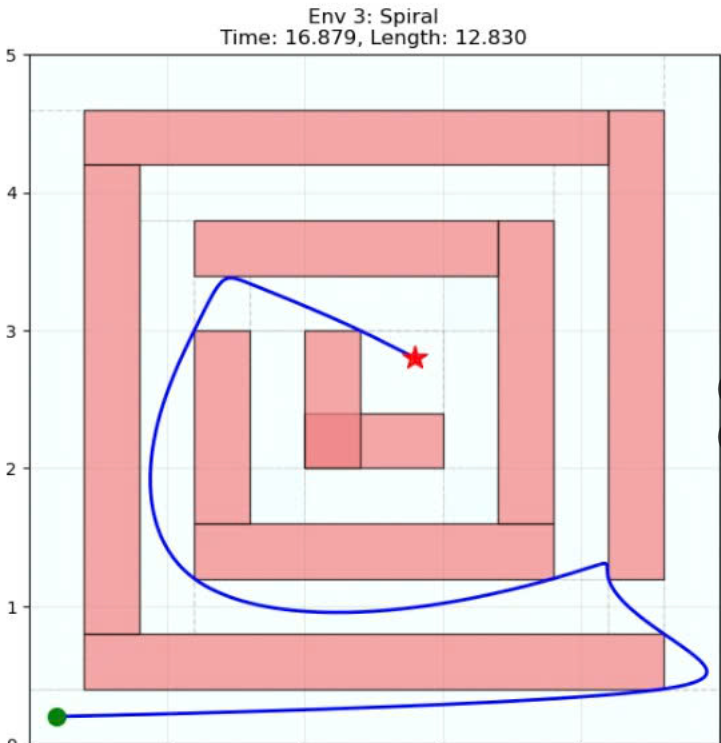
\includegraphics[width=0.8\textwidth]{../imgs/bezier-env3-1.png}
%             \caption{}
%         \end{figure}
%     \end{columns}
% \end{frame}
    
\begin{frame}{Demo 1: Maze}
    \begin{columns}[c]
        \column{0.5\textwidth}
        \begin{figure}
            \centering
            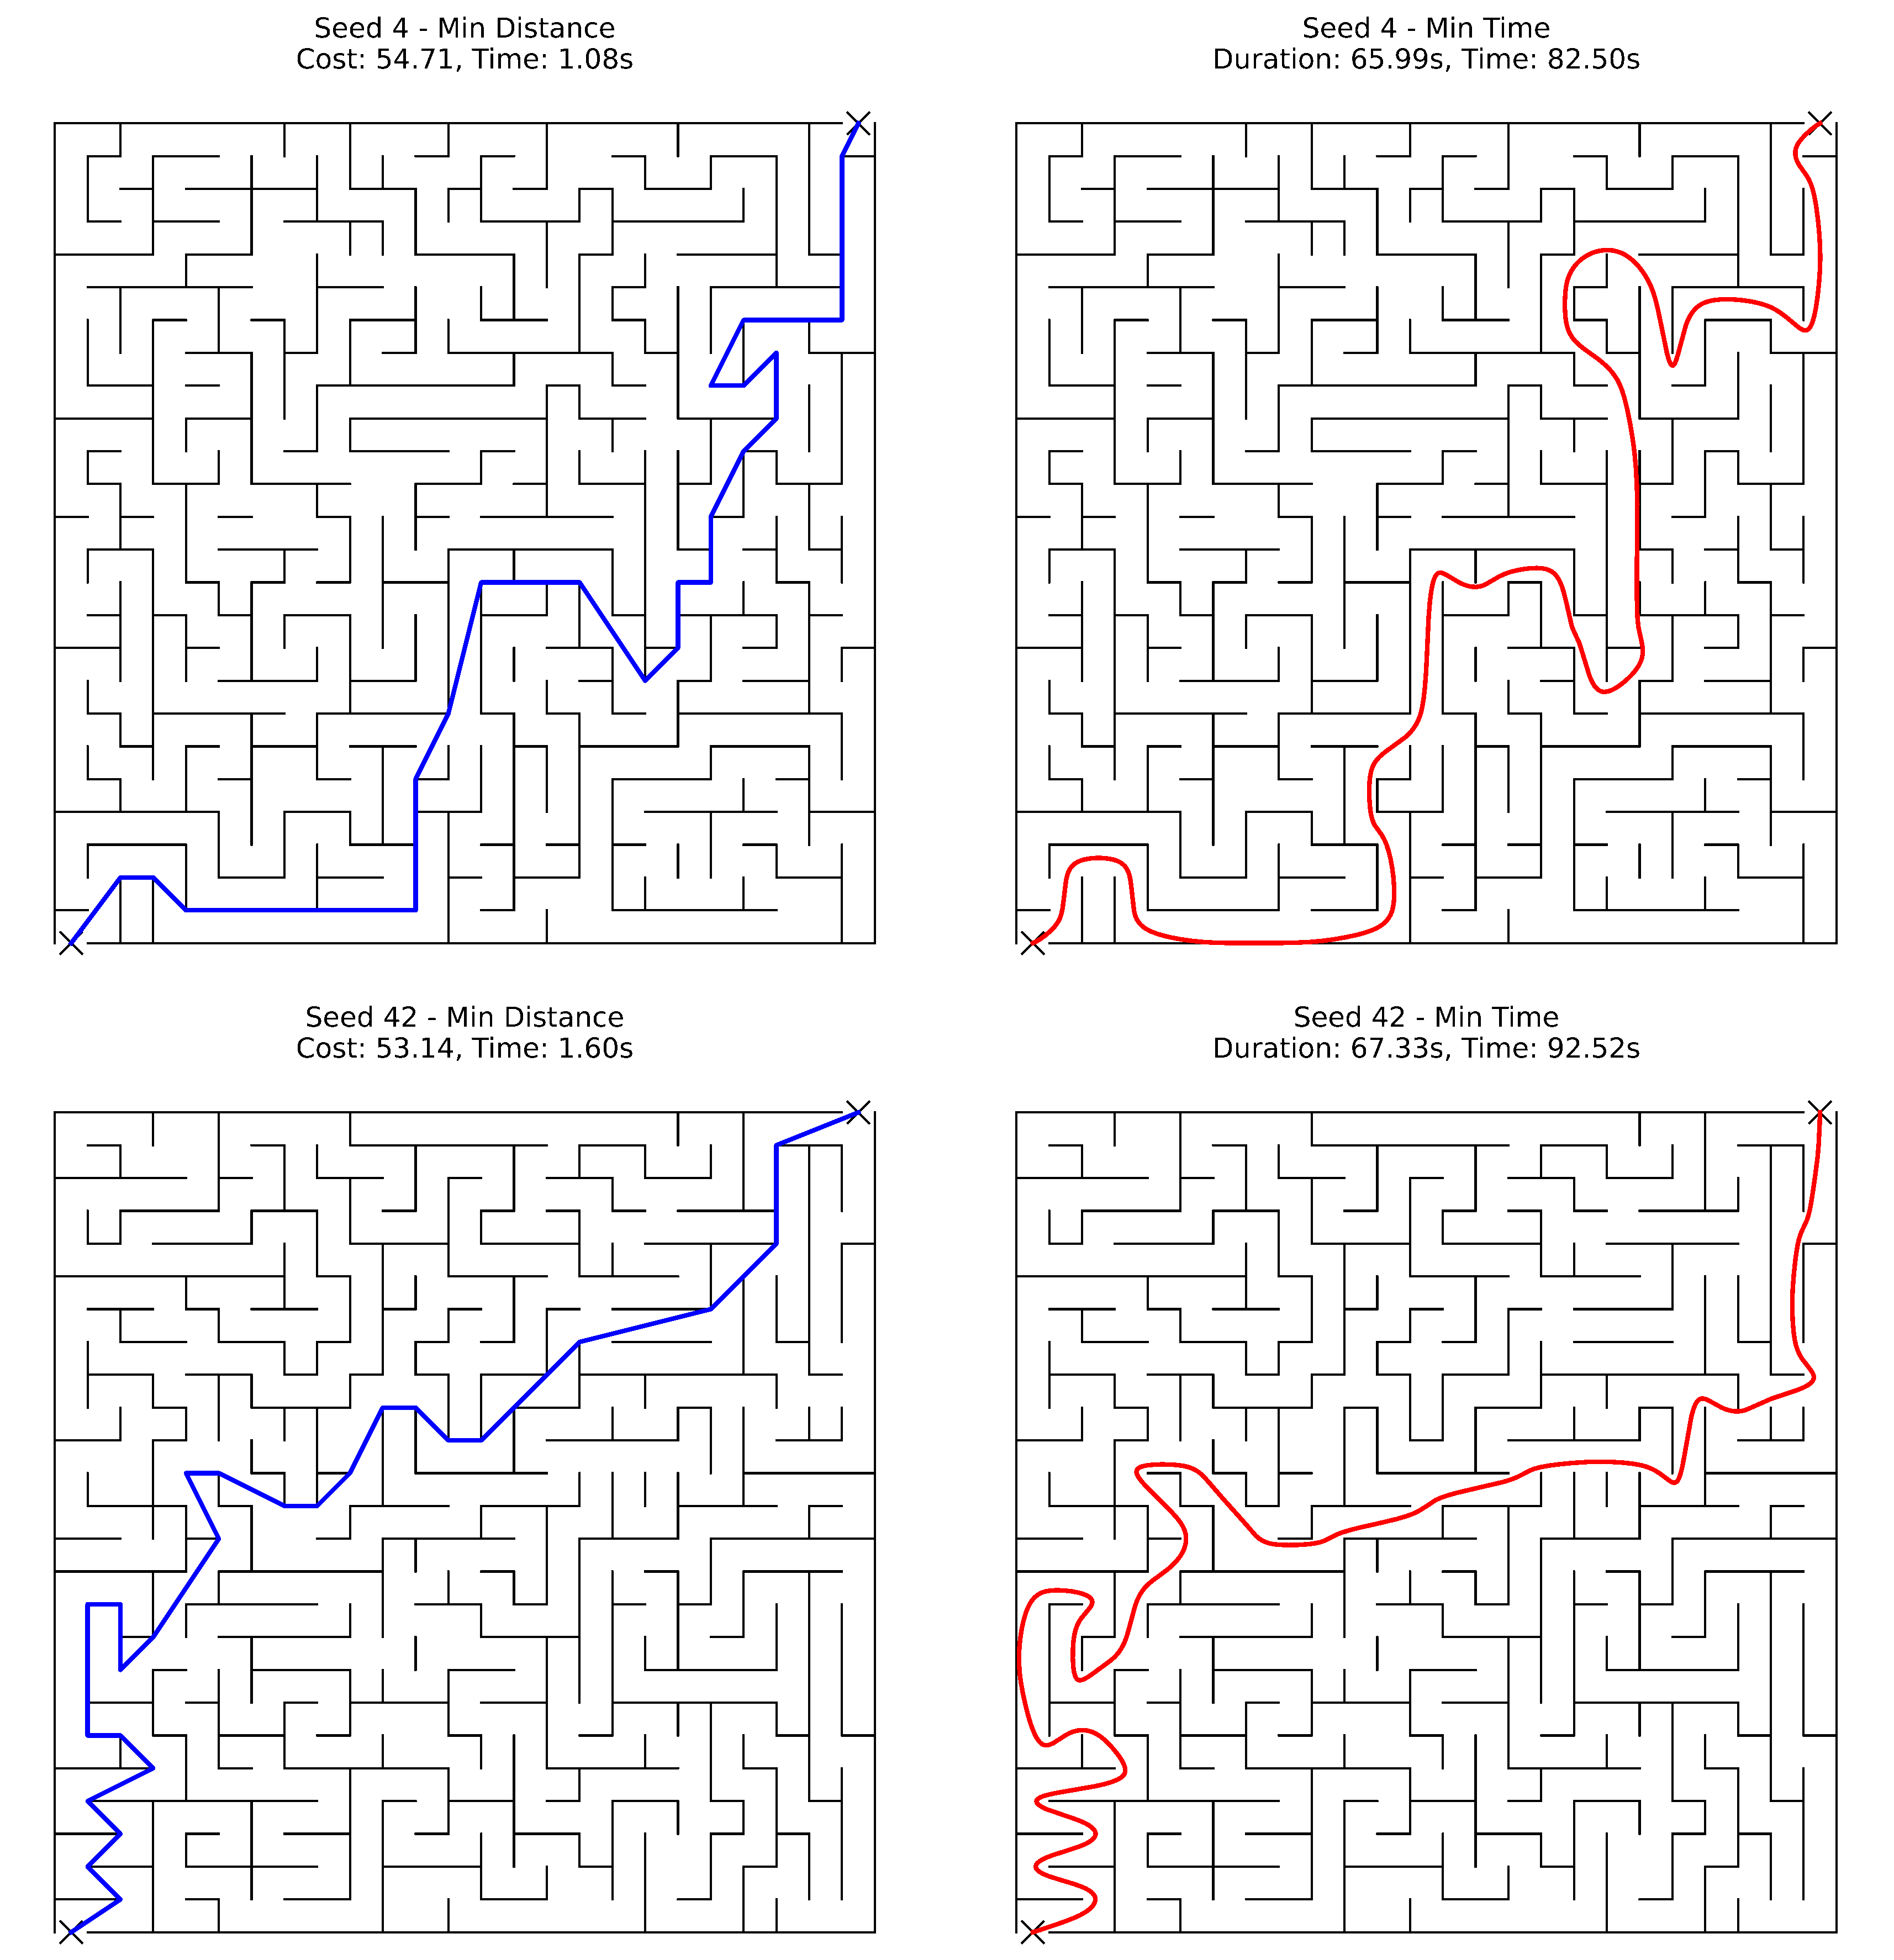
\includegraphics[width=0.8\textwidth]{../imgs/maze-1.png}
            \caption{}
        \end{figure}
        
        \column{0.5\textwidth}
        \begin{figure}
            \centering
            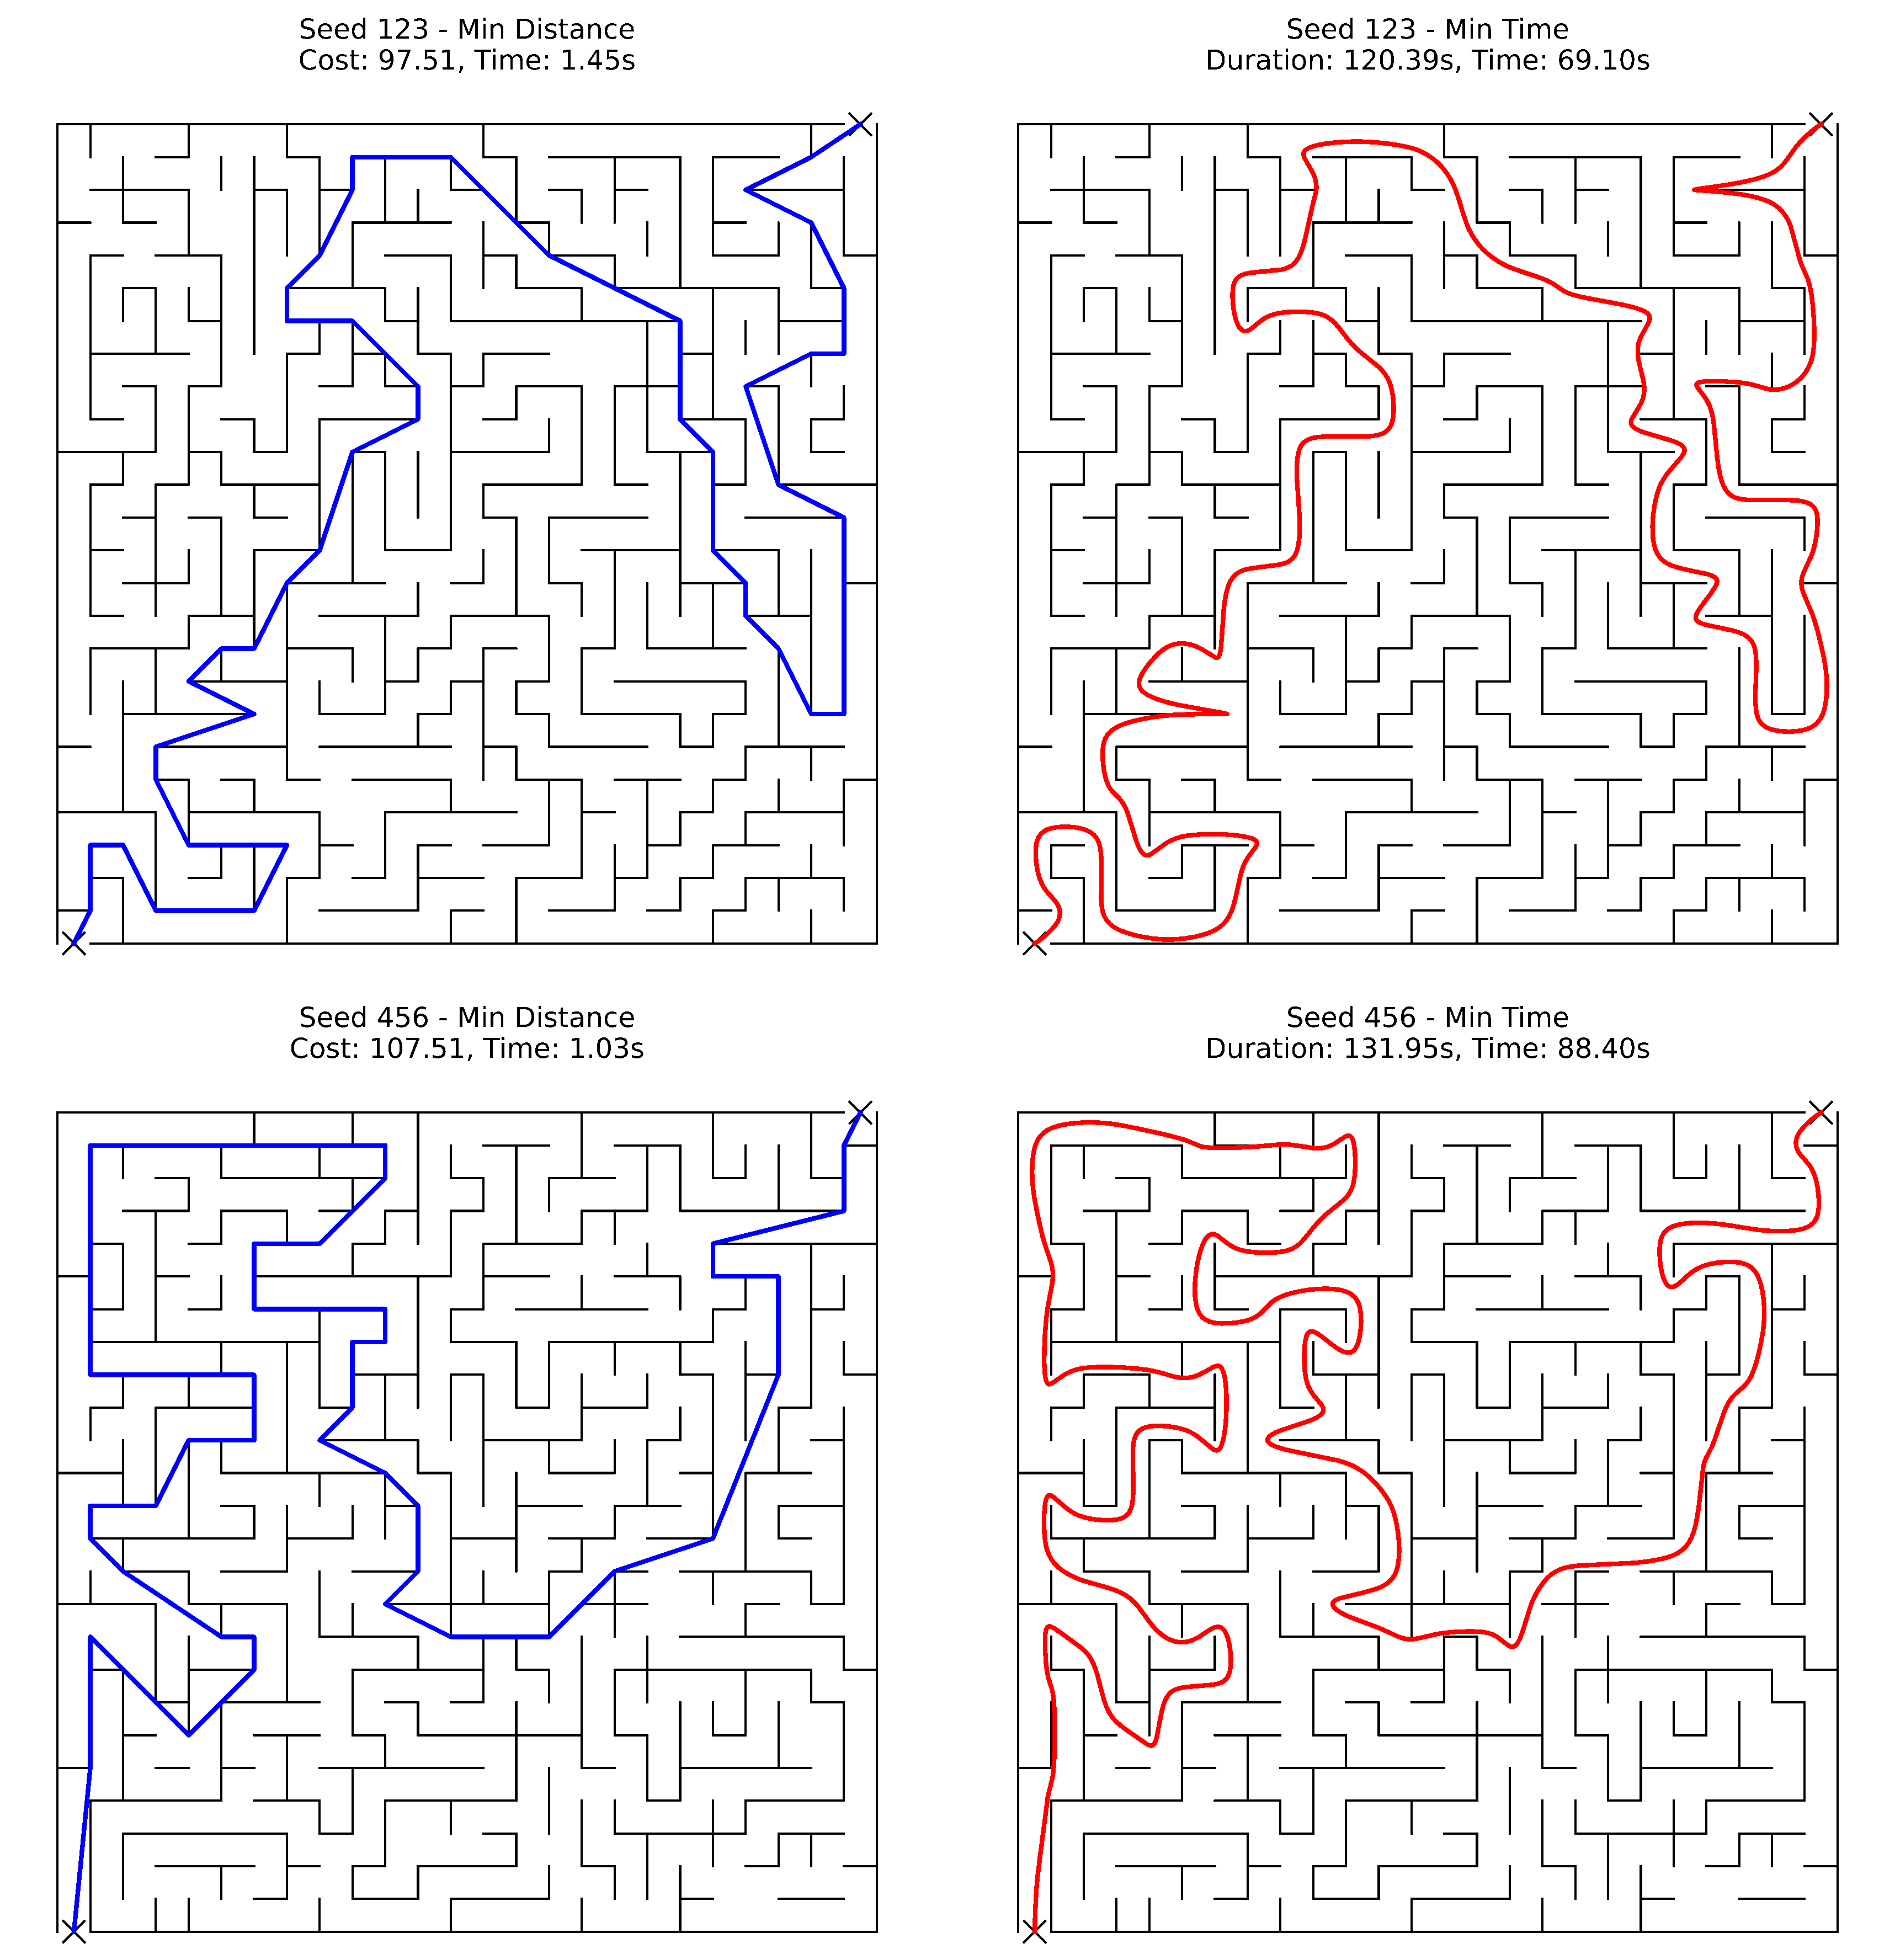
\includegraphics[width=0.8\textwidth]{../imgs/maze-2.png}
            \caption{}
        \end{figure}
    \end{columns}
\end{frame}

\begin{frame}{Demo 2: 2D Env}
    \begin{figure}
        \centering
        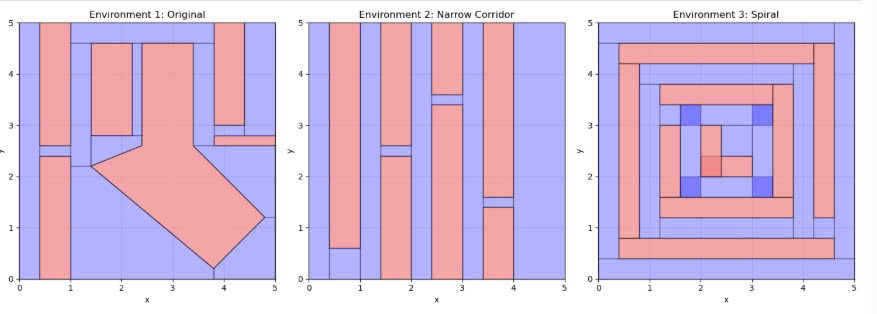
\includegraphics[width=0.75\textwidth]{../imgs/3env-2d.png}
        \caption{}
    \end{figure}
\end{frame}

\begin{frame}{Demo 2: 2D Env}
    \begin{figure}
        \centering
        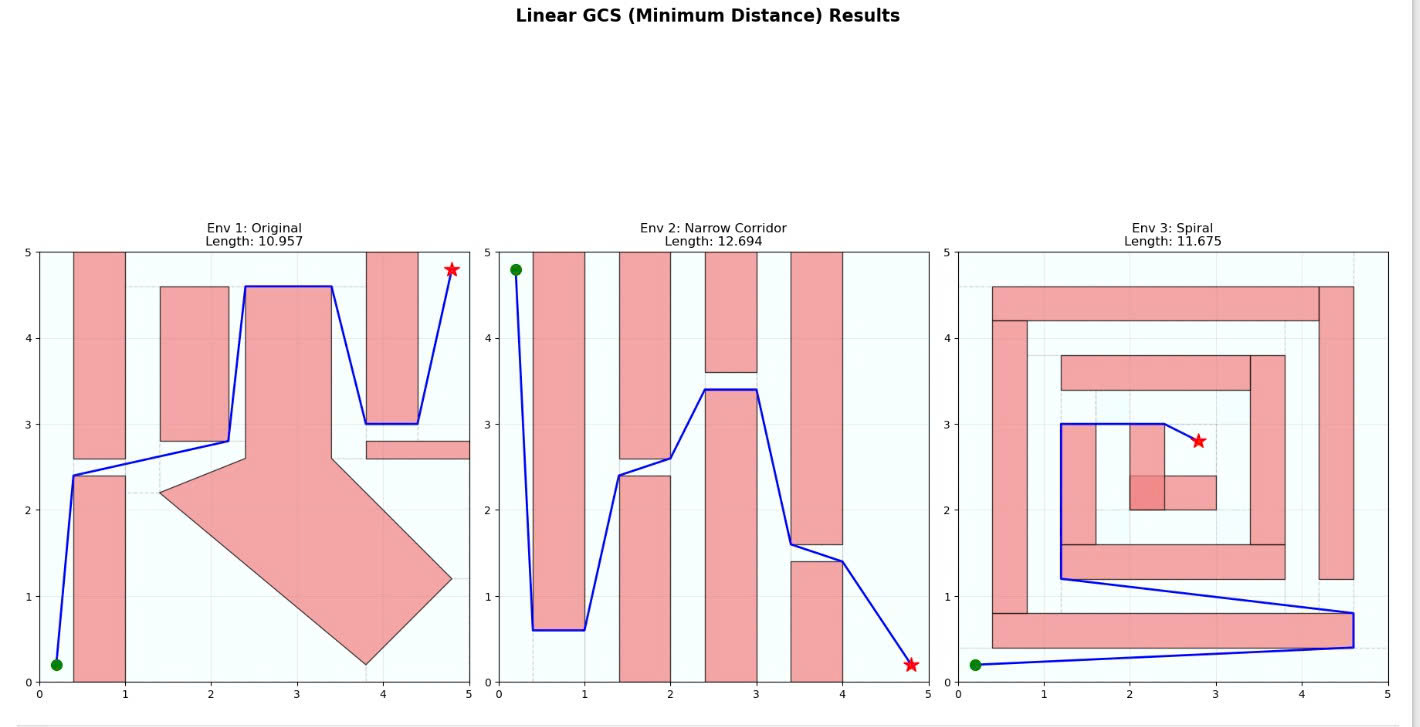
\includegraphics[width=0.75\textwidth]{../imgs/3env-2d-min-dis.png}
        \caption{}
    \end{figure}
\end{frame}

\begin{frame}{Demo 2: 2D Env}
    \begin{figure}
        \centering
        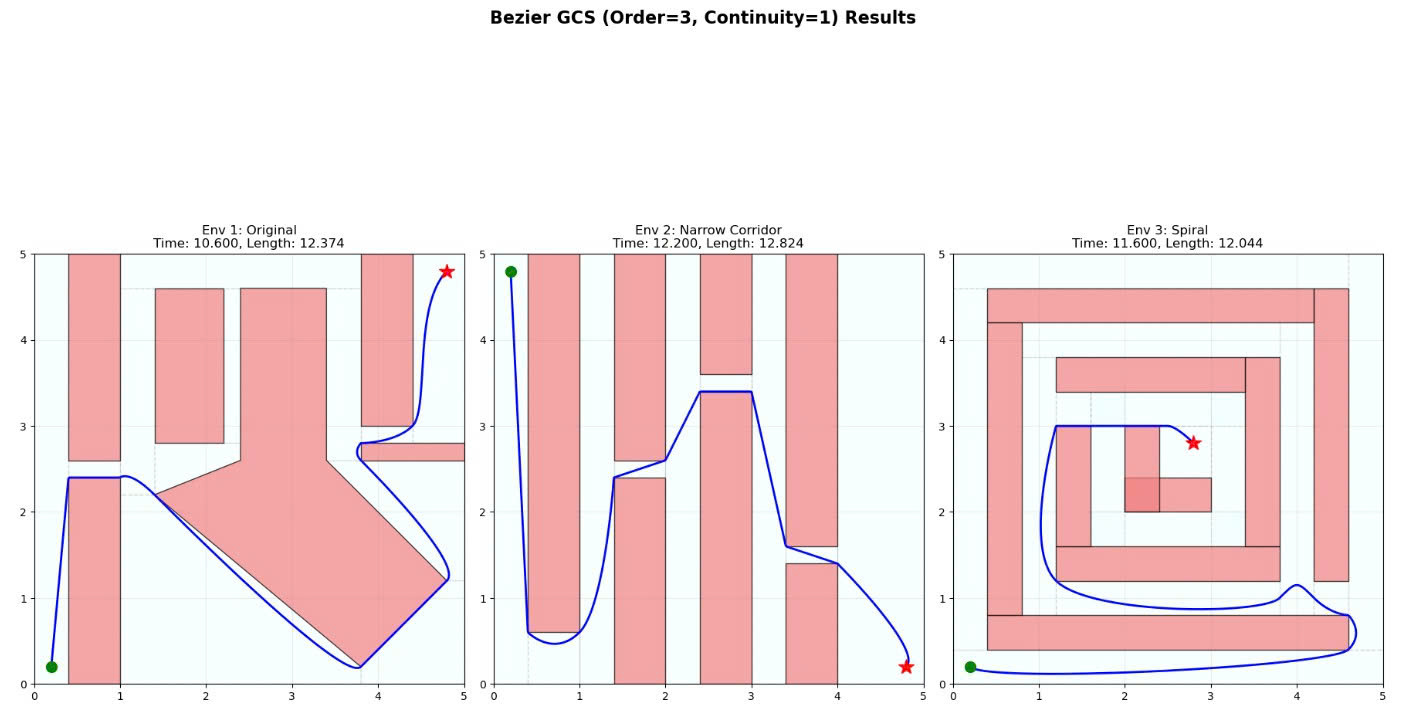
\includegraphics[width=0.75\textwidth]{../imgs/3env-2d-min-time.png}
        \caption{}
    \end{figure}
\end{frame}

\begin{frame}{Demo 3: Drone}
    % \begin{figure}
    %     \centering
    %     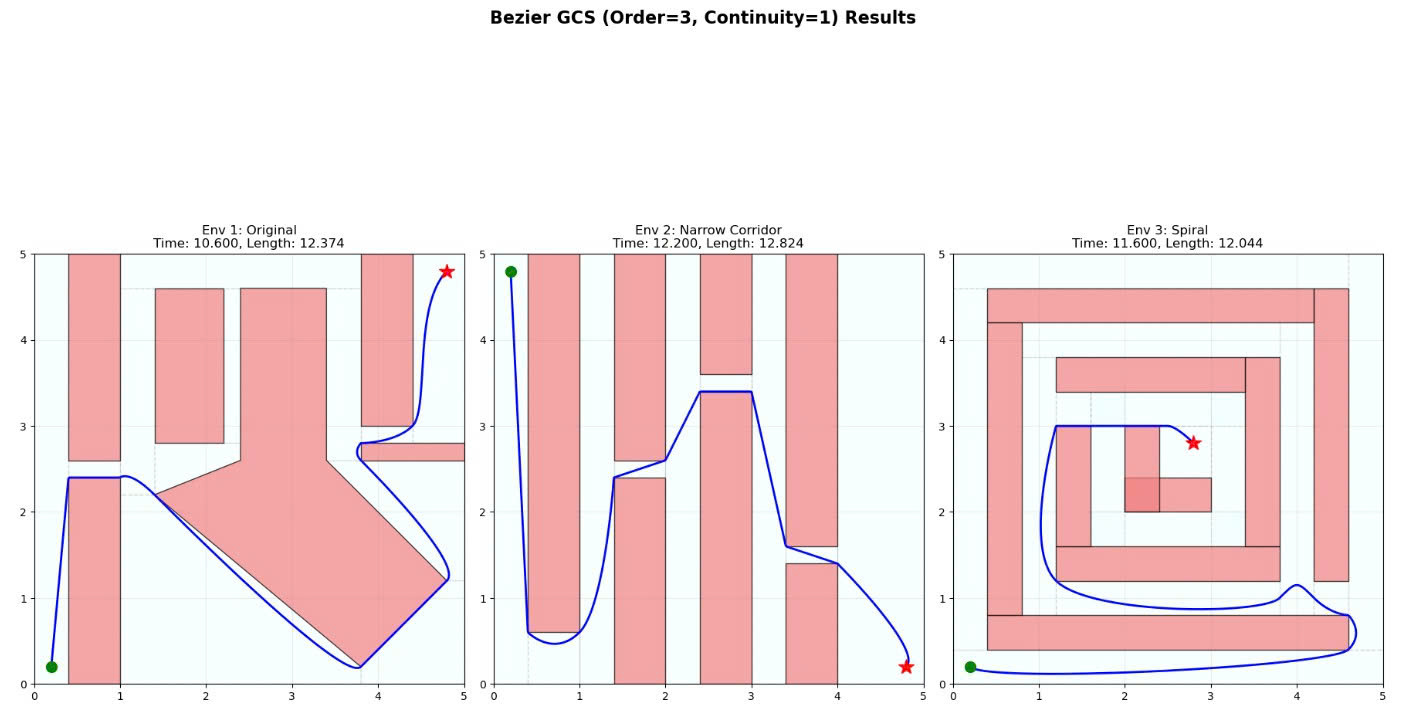
\includegraphics[width=0.75\textwidth]{../imgs/3env-2d-min-time.png}
    %     \caption{}
    % \end{figure}
    Video demo.
\end{frame}

\begin{frame}{Demo 4: Manipulation robot}
    % \begin{figure}
    %     \centering
    %     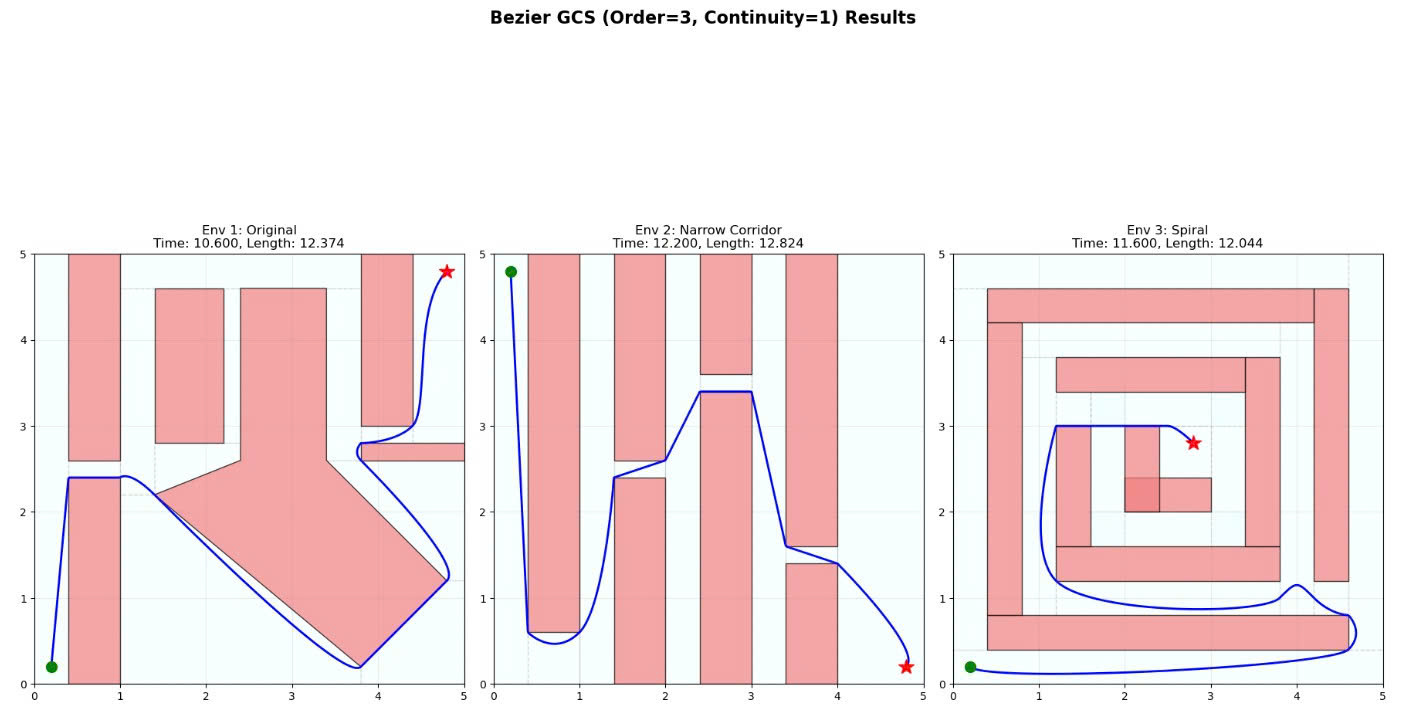
\includegraphics[width=0.75\textwidth]{../imgs/3env-2d-min-time.png}
    %     \caption{}
    % \end{figure}
    Video demo.
\end{frame}

\end{document}